% Very simple template for lab reports. Most common packages are already included.
\documentclass[a4paper, 11pt]{article}
\usepackage[utf8]{inputenc} % Change according your file encoding
\usepackage{graphicx}
\usepackage{url}
\usepackage{listings}
\usepackage[listings]{tcolorbox}
\usepackage{xcolor}
\usepackage{float}
\usepackage{placeins}

% Define a custom boxed listing environment
\newtcblisting{mylisting}{
  colback=gray!5!white, colframe=black!75!white,
  listing only,
  left=2mm, right=2mm, top=1mm, bottom=1mm,
  boxrule=0.5pt, arc=2mm
}

%opening
\title{Report 3 - Routy: A Logical Time Logger}
\author{Lorenzo Deflorian}
\date{\today{}}

\begin{document}

\maketitle

\section{Introduction}

The main goal of this assignment was to implement a logger that uses logical time to order messages in a distributed system. The logger should be able to handle messages that are received out of order and log them in the correct order based on their logical timestamps.

For this purpose, I implemented both a Lamport clock and a vector clock. The Lamport clock is a simple counter, starting from 0, that is incremented every time a message is sent or received. The vector clock is a map that keeps track of the logical time of each node in the system. Every time a message is sent, the sender increments its own clock and includes the updated clock in the message. When a message is received, the receiver updates its own clock by taking the element-wise maximum of its own clock and the received clock.

To log the messages in the correct order, I also implemented a holdback queue that stores messages considered unsafe to log. A message is considered safe to log if its timestamp is less than or equal to all the timestamps that the logger keeps track of. At each iteration, the logger checks the holdback queue for any messages that can be logged and logs them in the correct order.


\section{Main problems and solutions}

\subsection{Logging in the wrong order}

After implementing the basic functionality of the logger, running the test with a high jitter (300 ms) immediately showed that without a holdback queue the logger could not log messages in the correct order. This can be easily seen by looking for entries like the following in the log file:
\begin{tcolorbox}[colback=black!5!white, colframe=black!80!white, title=Log Output, fonttitle=\bfseries, sharp corners=south, listing only]
\begin{verbatim}
log: 2 george {received,{hello,83}}
log: 1 paul {sending,{hello,83}}
log: 4 john {received,{hello,15}}
log: 2 paul {sending,{hello,93}}
log: 5 john {received,{hello,53}}
log: 3 george {sending,{hello,15}}
log: 4 george {received,{hello,93}}
log: 1 ringo {sending,{hello,53}}
log: 6 john {received,{hello,30}}
log: 8 george {received,{hello,81}}
log: 10 ringo {received,{hello,12}}
log: 3 paul {sending,{hello,30}}
log: 7 john {sending,{hello,81}}
log: 9 george {sending,{hello,12}}
log: 11 ringo {received,{hello,35}}
log: 11 john {received,{hello,29}} <--- OUT OF ORDER
log: 4 paul {sending,{hello,35}}
log: 13 john {received,{hello,74}}
log: 10 george {sending,{hello,29}} <--- OUT OF ORDER
log: 15 paul {received,{hello,24}}
log: 11 george {sending,{hello,69}}
log: 12 ringo {sending,{hello,74}}
log: 14 john {sending,{hello,24}}
log: 15 john {received,{hello,69}}
log: 16 john {received,{hello,25}}
\end{verbatim}
\end{tcolorbox}

As we can see by pairing the sending and receiving messages, the order is not respected for the message \{hello,29\}, which is first received and then sent.

\begin{table}[H]
\centering
\begin{tabular}{|l|l|c|l|c|c|}
\hline
\textbf{Message} & \textbf{Sender} & \textbf{Send Time} & \textbf{Receiver} & \textbf{Receive Time} & \textbf{Ordered?} \\
\hline
\{hello,83\}  & paul   & 1  & george & 2  & Yes \\
\{hello,15\}  & george & 3  & john   & 4  & Yes \\
\{hello,93\}  & paul   & 2  & george & 4  & Yes \\
\{hello,53\}  & ringo  & 1  & john   & 5  & Yes \\
\{hello,30\}  & paul   & 3  & john   & 6  & Yes \\
\{hello,81\}  & john   & 7  & george & 8  & Yes \\
\{hello,12\}  & george & 9  & ringo  & 10 & Yes \\
\{hello,35\}  & paul   & 4  & ringo  & 11 & Yes \\
\{hello,74\}  & ringo  & 12 & john   & 13 & Yes \\
\{hello,29\}  & george & 10 & john   & 11 & No  \\
\{hello,69\}  & george & 11 & john   & 15 & Yes \\
\{hello,24\}  & john   & 14 & paul   & 15 & Yes \\
\hline
\end{tabular}
\caption{Message send and receive times with validity}
\end{table}

Even though the send and receive are logged in the wrong order, the timestamps respect causality. This means that the logical clocks are working correctly.

\subsection{Hold My Logs}

I implemented a holdback queue to store unsafe messages and only log the safe ones. At the beginning of each iteration the logger checks the holdback queue for any messages that can be logged and logs them in the correct order. When the logger receives a message it checks whether the message is safe to log; if it is, the logger logs it, otherwise it adds it to the holdback queue. When the logger receives a stop message, it logs all remaining messages in the holdback queue.

Below is a plot showing how many messages are stored in the holdback queue during the execution of the test with high jitter (300 ms) across 50 nodes. Note that for this test I modified the message ID to be a random number between 1 and 1,000,000 instead of between 1 and 100 to reduce the probability of two messages having the same ID.

\begin{figure}[H]
  \centering
  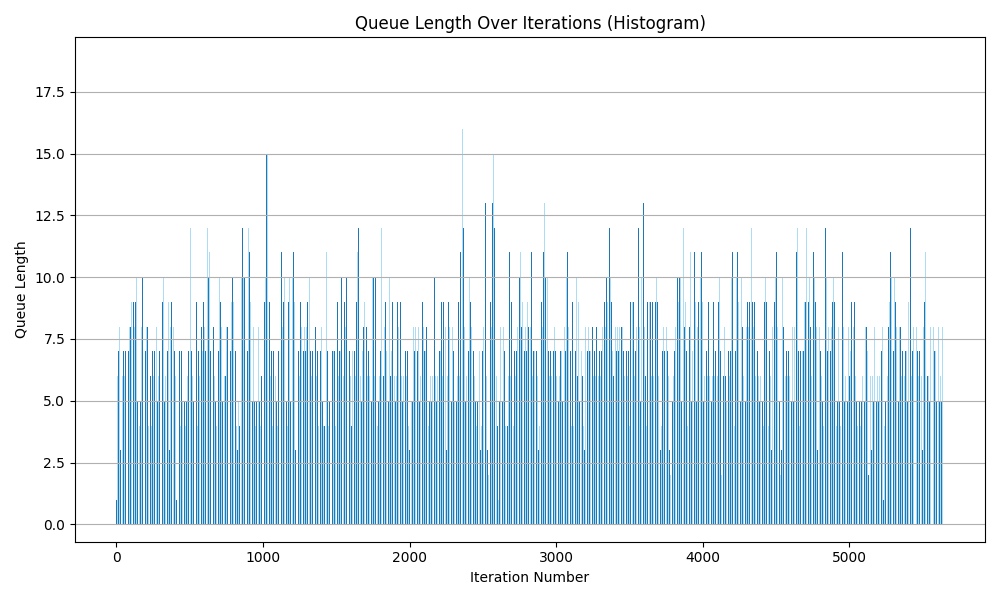
\includegraphics[width=0.8\textwidth]{imgs/test_queue_len_50_histogram.png}
  \caption{Histogram of holdback queue length during execution with 50 nodes and 300 ms jitter}
  \label{fig:queue_histogram}
\end{figure}

As shown in figure \ref{fig:queue_histogram}, the holdback queue length is mostly between 0 and 5 messages, with a few peaks reaching up to 17 messages. This indicates that the logger is able to log most messages in the correct order without storing them in the holdback queue for long.

\subsection{V for Vector}
To further improve the logging order, I implemented a vector clock. The vector clock is a map that keeps track of the logical time of each node in the system. Every time a message is sent, the sender increments its own clock and includes the updated clock in the message. When a message is received, the receiver updates its own clock by taking the element-wise maximum of its own clock and the received clock.

Using the script \texttt{check_vector.py}, I verified that the vector clock is working correctly and that messages are logged in the correct order.

Sometimes a message appears to be received without having been sent first. This happens because of the jitter introduced between the Send and the Log call. Nevertheless, this does not affect the correctness of the logging order or the causality of the messages.

\section{Conclusions}

In summary, I implemented a logger that uses logical time to order messages in a distributed system. The logger handles messages received out of order and logs them in the correct order according to their logical timestamps. The implementation of a holdback queue and a vector clock further improves the logging order and ensures that messages are logged in a causally consistent manner.

\end{document}
